\section{Limits}
\subsection{A First Example}
Our point of departure is the familiar equality 
\[\label{eq:onethird}
\frac{1}{3} = 0.333\cdots\ 
\]
where the dots mean that the decimal goes on forever repeating the digit ``3". We take this for granted, but really there is something odd here; infinity is a rather profound concept, so why do we need an infinitely long number -- something nobody could ever even write down! -- to express something as straightforward as dividing one by three? The answer is that we have no choice: any finite sequence of 3s is too small, but as soon as we write a 4 it is too large. There is no finite decimal which comes out to \emph{exactly} one-third. 

When using numbers to measure things, this is not a problem, because physical measurements are never exact. How many decimal places we care about depends entirely upon what we are doing. For a carpenter cutting a board, there is no meaningful difference between 0.33 inches and a third of an inch; if we are guiding a spacecraft there is no real difference between $\frac{1}{3}$ kilometer and 0.3333333 kilometers, as these differ by less than the width of a hair. So in general we do not need many decimal places to get \emph{very} close. There is no way to put a strict bound on the largest number of decimal places we might ever need, but no matter how much accuracy we seek, we can always get there. 

This notion of a sequence of ever-better approximations, which can eventually attain any required level of accuracy, is in fact the essential idea which will be the basis for everything we do in calculus. Before diving into general definitions, we will restate more precisely what we mean by  ``approximation". When we assert that $0.333\cdots = \frac{1}{3}$, what we are really claiming is this:

\begin{thm}\label{thm:onethird}
Let $\varepsilon$ be any number greater than 0. There exists some integer $N$ such that
\[
\frac{1}{3} - 0.\underbrace{33\cdots3}_\text{$N$ times} < \varepsilon 
\]
\end{thm}

The idea here is that $\varepsilon$ is the required ``degree of accuracy", or ``error tolerance" for our approximation. We must exclude $\varepsilon=0$ because that would mean perfect accuracy -- which is not possible. But anything short of perfection is possible -- which is why we can say \emph{any} $\varepsilon>0$. 

We prove our claim in the straightforward way -- by explicitly calculating the required number of digits $N$ (which depends on $\varepsilon$). Smaller $\varepsilon$ means more accurate approximation, which requires larger $N$. To start we can get rid of fractions (often a good thing to do when manipulating algebraic expressions) by multiplying both sides of the inequality by 3; now we have to find $N$ such that
\[
1 - 0.\underbrace{99\ldots9}_\text{$N$ times}  < 3\varepsilon 
\]
i.e
\[
10^{-N} < 3\varepsilon 
\]
And of course we can always find such an $N$; if the decimal expansion of $3\varepsilon$ starts with, say, 47 zeros, take $N>47$ and so on. 

The important thing about this proof is that the vague notation ``$\cdots$" is gone; we have stated everything in terms of inequalities involving finite expressions. The only point at which infinity enters the picture is in considering \emph{all} of the infinitely many finite expressions we could imagine writing.  This typifies the kind of reasoning we will use to deal with infinity. 

We should note that the ``infinity" of $0.33\ldots$ is avoidable and somewhat artificial, since we already have a perfectly good finite way of writing down this quantity, i.e. ``$1/3$". \footnote{And if we used base-3 instead of base-10, we would write this number finitely as ``0.1".}
Reasoning about infinity will become truly essential when we consider numbers that inherently cannot be represented as fractions,  like $\sqrt{2}=1.4142135623730951\cdots$ or  $\pi = 3.1415926\cdots$.\footnote{If the fact that these numbers cannot be fractions is unfamiliar to you, see section \ref{sec:sqrtIrrational}}

\subsection{Exercises}
\begin{enumerate}
\item In the same manner as Theorem \ref{thm:onethird}, prove that
	\begin{itemize}
	\item $1/9 = 0.11111\ldots$
	\item $1/7=0.142857142857142857\ldots$
	\end{itemize}
\item Considering the previous exercise, how might you figure out the decimal expansion of $1/11$ without a calculator?
\item Express .027027027... as a fraction. 
\end{enumerate}


\subsection{Definition of Limits}
So far we have considered approximations stated in terms of ever-longer decimal expansions, but that is just because decimals are  familiar and easy to deal with. In fact there is nothing special, or even particularly important, about decimal expansions. Certainly the sequence $3.1, 3.14, 3.141, \ldots$ keeps getting closer to $\pi$, but there are many other ways to get there. One well-known approximation starts with $\frac{22}{7}$, followed by $\frac{333}{106}$, then $\frac{355}{113}$; we are not ready yet to explain where these numbers come from, but you can do the division and see that these fractions are close to the familiar $3.1415926\cdots$.

We have been speaking informally about ``sequences" of numbers, but since these will be so important we need a definition. A sequence is an infinite ordered list of real numbers, usually written with subscripts to show where in the list we are: $a_0,a_1, a_2, a_3 \cdots$ et cetera (whether we start at one or zero does not much matter, but more often we start at zero). More formally, a sequence is a function mapping the natural numbers to the real numbers.

We now state our most fundamental definition, which generalizes the concept behind theorem (\ref{thm:onethird}):
\begin{defn}\label{def:limit}
Let $a_0,a_1,a_2,\ldots$ be a sequence of real numbers. The real number $A$ is the \emph{limit} of this sequence if,
for each $\varepsilon > 0$, there exists an integer $N_\varepsilon$ such that
\[
|A - a_n| < \varepsilon 
\]
whenever $n \geq N_\varepsilon$. We write this as
\[
\lim a_n = A
\]
\end{defn}
We use absolute value because it does not matter whether $a_n$ is smaller or larger than $A$, all that matters is that they are in some sense \emph{close}; the absolute value gives us the \emph{distance} between two numbers, which is what we need. 

%I do not think we have actually used this language anywhere -- will we?
%Whenever there is an $N$ such that some proposition $P(n)$ holds whenever $n>N$, we may say that ``$P(n)$ is eventually true" or, more tersely, ``eventually $P(n)$". The use of the word ``eventually" suggests the passage of time; in general there is no reason why larger $n$ in $a_n$ has to refer to  later moments in time, but it is often natural to think of things this way, as if the terms of a sequence are being revealed in order.

A sequence which has a limit is said to \emph{converge}, or to be convergent; a sequence which does not converge is \emph{divergent}. So theorem (\ref{thm:onethird}) can be restated as asserting that the sequence
\[
a_n = \frac{3}{10} + \frac{3}{100} + \cdots + \frac{3}{10^n}
\]
converges to $1/3$, i.e. that $\lim a_n = 1/3$.
Note that $a_n$ is defined as the sum of the first $n$ terms of yet another sequence (i.e. $b_k=\frac{3}{10^k}$); we will see in the next chapter that many other sequences are defined in this way.

We will see many examples of sequences which do and do not converge, and will use convergence as the basis for other definitions. But first we give another example of how to find the limit of a sequence.

\begin{thm}\label{thm:oneOverN}
Let $a_n = \frac{1}{n}$. Then
$\lim a_n = 0$.
\end{thm}
We usually simplify the notation and just write this as $\lim \frac{1}{n} = 0$.
We must prove that, for any $\varepsilon > 0$, we have 
\[
|0 - 1/n| < \varepsilon
\]
when $n$ is larger than some yet-to-be-determined $N_\varepsilon$. This can be written more simply as
\[
1/n < \varepsilon
\]
and so 
\[
n > 1/\varepsilon
\]
Thus we take  $N_\varepsilon$ to be (at least) the next integer past $1/\varepsilon$ (which will be large when $\varepsilon$ is small).

Not every sequence of numbers has a limit; a sequence like $a_n=(-1)^n$ (i.e. 1,-1,1,-1,1,$-1\cdots$) that bounces around rather than settling down close to one particular value is a good example.
To prove this, we must show that no real number could satisfy our definition.
For instance we cannot have $\lim a_n =1$; taking $\varepsilon = 1/2$, no matter how large $N$ is there will always be $n>N$ for which $a_n = -1$ so $|a_n - 1| > 1/2$.
All other numbers can be dismissed similarly.%\footnote{With this you have reached a true epoch in your mathematical education; problems for which it is not always easy to figure out if there even is an answer. You might want to mark this occasion with appropriate ceremony. But please no underage drinking.}

A sequence can also fail to have a limit by going off to infinity, for instance $a_n=n$. No real number $X$ could be the limit; for any $\varepsilon$ we will have $a_n>X+\varepsilon$ if $n>X+\varepsilon$.

\subsection{Exercises}
\begin{enumerate}
\item Finish the proof that  $(-1)^n$ does not have a limit
\item Prove that $\lim 17/n^2 = 0$
\item Evaluate $\lim \frac{n-42}{2n-1}$
\item Restate the results from the first set of exercises in terms of limits.
\end{enumerate}


The proof of theorem \ref{thm:oneOverN} actually merits a bit more scrutiny.
We have taken it for granted that, for every real number (the real number $1/\varepsilon$ in this case), there exists a larger \emph{integer}; this is called the ``Archimedean property" of the real number system.
This seems rather obvious and is indeed true; it is another way of saying there are no ``infinitely large" numbers that cannot be reached with a finite number of fixed-size steps\footnote{It also means there are no ``infinitessimally small" numbers that cannot be added up to reach something large.}. 
But it is an assumption and should be explicitly identified as such, along with more familiar assumptions like the commutative and distributive properties. We will see other results that require the Archimedean property later in the chapter.

\subsection{Exercises}
\begin{enumerate}
\item The proof that $a_n=n$ diverges also implicitly used the Archimedean property; where?
\item Prove that $\lim 17/n^2 = 0$
\item Evaluate $\lim \frac{n-42}{2n-1}$%need to show example of n/(n+1)
%\item $\lim nx^n = 0$ for any $x$ such that  $|x|<1$.
\item $\lim \frac{n^2}{2^n} = 0$
\end{enumerate}


\subsection{Basic Properties of Limits}
To work with limits we will need to establish some of their  basic properties. We will put the possibility of non-convergence aside for the moment, and focus on what must be true about limits when they do exist. The most fundamental property of limits is that they are \emph{unique}: given $a_n$, if there is \emph{any} number $A$ satisfying definition (\ref{def:limit}), then there is only one such number. This is why we always speak of \emph{the} limit of a sequence. 

\begin{thm}\label{thm:uniqueness}
Suppose that $A$ is a limit of $a_n$ -- i.e. that $A$ and $a_n$ satisfy definition (\ref{def:limit}). Then no other number is a limit  of $a_n$.\end{thm}

\begin{proof}
Let $B\neq A$; we must show that $B$ is \emph{not} a limit of $a_n$. The idea is to make $\varepsilon$ smaller than the gap between $A$ and $B$. By definition, once $n$ gets large enough the sequence will then stay in the open  interval\footnote{If you have not encountered this term before, the \emph{open} interval $(a,b)$ is the set of all numbers between $a$ and $b$, \emph{excluding} the endpoints $a,b$. If we include the endpoints we have a \emph{closed } interval, written $[a,b]$} $(A-\varepsilon,A+\varepsilon)$; that is just another way of saying $|a_n-A|<\varepsilon$. Since $B$ is outside this interval, the sequence will not stay ``close" to $B$ when $n$ is this large. Now let us work through this idea more carefully. 

Choose $\varepsilon, \varepsilon'$ so that the intervals $(A-\varepsilon,A+\varepsilon)$,   $(B-\varepsilon',B+\varepsilon')$ do not overlap. It is clearly possible to do this; looking at diagram (\ref{fig:uniqueness}), we can see that what we require is $\varepsilon+\varepsilon' \leq |A-B|$.  Let $N$ be a number (known to exist by assumption) such that $n>N$ implies $|a_n-A|<\varepsilon$.  Now could there be an $N'$ such that $n>N'$ implies $|a_n-B|<\varepsilon'$? No! Whatever $N'$ is, we could have $n$ greater than \emph{both} $N'$ and $N$ -- i.e. $n>\max(N,N')$. Then we must have  $a_n \in (A-\varepsilon,A+\varepsilon)$, in which case $a_n \not\in (B-\varepsilon',B+\varepsilon')$. The non-existence the required $N'$ means that $B$ is not a limit of $a_n$.
\end{proof}

\begin{figure}
\begin{center}
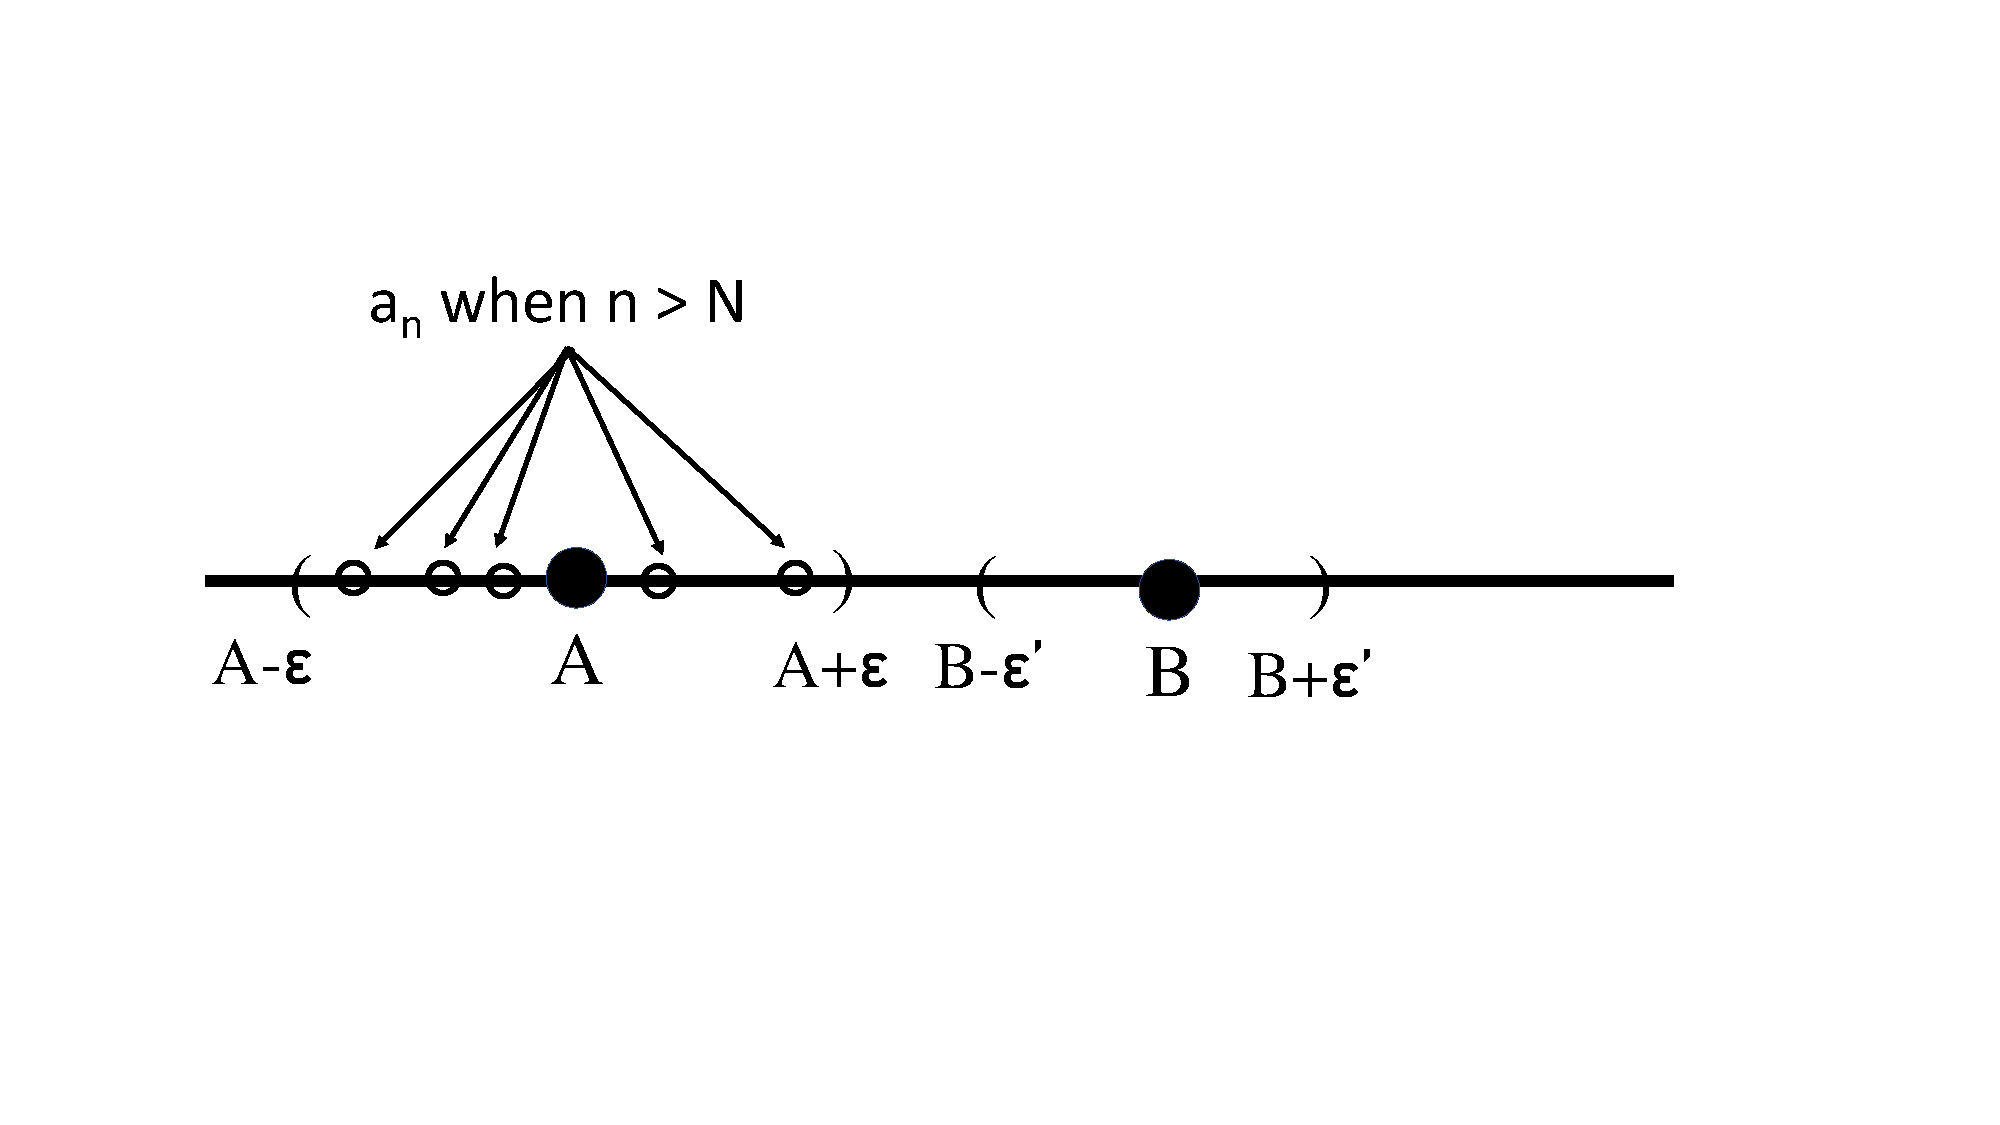
\includegraphics[scale=0.25]{uniqueness}
\end{center}
\caption{Proof of Theorem (\ref{thm:uniqueness})\label{fig:uniqueness}}
\end{figure}

The next theorem, as well as the following exercises, show how we can evaluate complicated limits by breaking them down into smaller parts.
\begin{thm}\label{thm:sumOfLim}
If $a_n,b_n$ are convergent with $\lim a_n=A$ and $\lim b_n=B$ then
\[
\lim (a_n + b_n) = A+B
\]  
\end{thm}
\begin{proof}
The idea here is that if $a_n$ is close to $A$ and $b_n$ is close to $B$ then their sum must be close to $A+B$, see figure \ref{fig:sumOfLim}. What we need to do is to determine how close is close enough to imply
\[
A+B-\varepsilon \leq a_n+b_n \leq A+B + \varepsilon \ .
\]
Whatever $\varepsilon>0$ may be, there will exist $\varepsilon_1>0, \varepsilon_2>0$ such that $\varepsilon_1 + \varepsilon_2 < \varepsilon$, and we have (by assumption) $N_1,N_2$ for which
\begin{align*}
A-\varepsilon_1 \leq a_n &\leq A+ \varepsilon_1 \ \mbox{ if } n > N_1\\
B-\varepsilon_2 \leq b_n &\leq B+ \varepsilon_2 \ \mbox{ if } n > N_2
\end{align*}
thus
\[
A+B-\varepsilon \leq a_n+b_n \leq A+B + \varepsilon \ .
\]
if $n$ is greater than both $N_1$ and $N_2$.

\end{proof}
\begin{figure}
\begin{center}
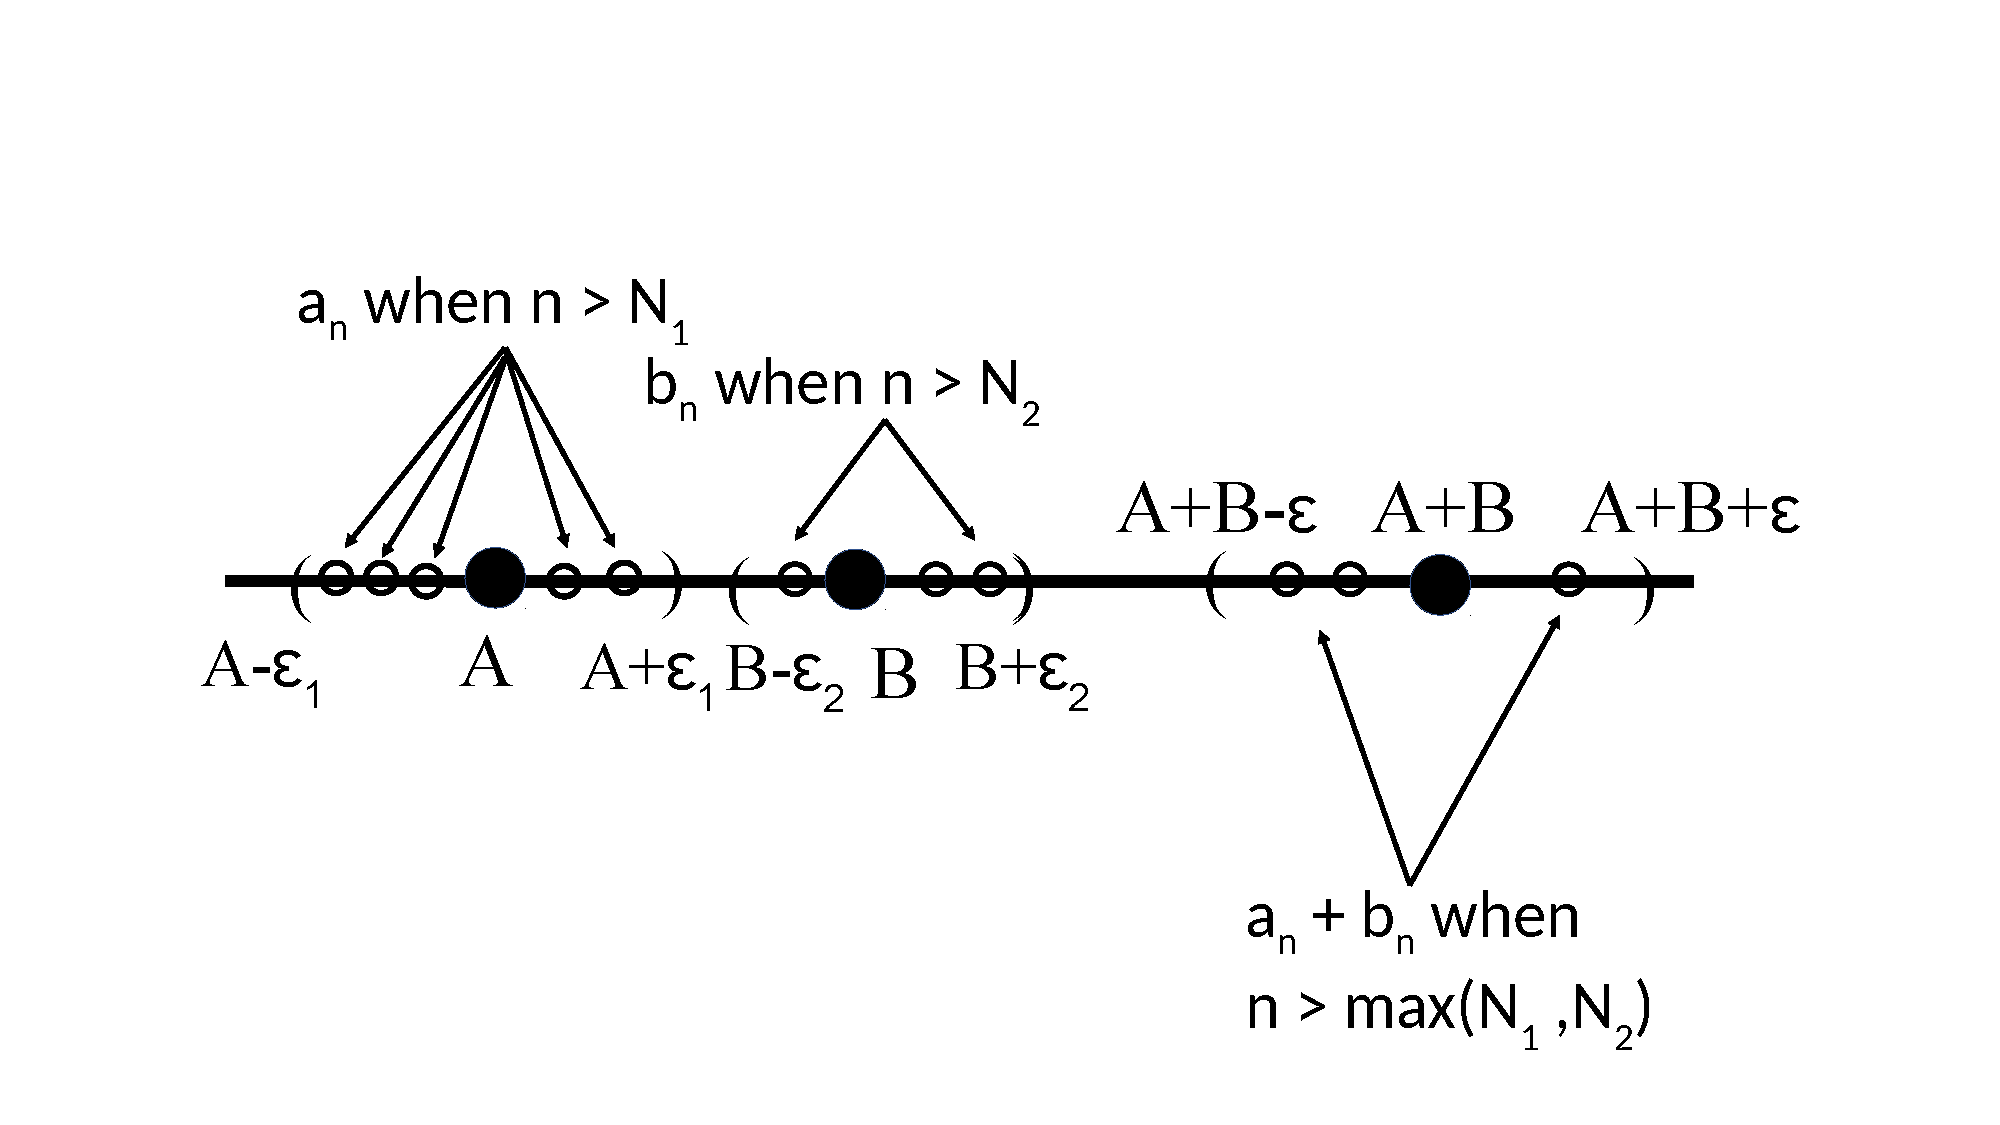
\includegraphics[scale=0.25]{sumOfLimits}
\end{center}
\caption{Proof of Theorem (\ref{thm:sumOfLim})\label{fig:sumOfLim}}
\end{figure}

In addition to manipulating sequences by performing algebraic operations on their terms, we can also ``thin out" a sequence by dropping some terms. The next theorem tells us that if $a_n$ converges, then sequences like $a_2,a_4,a_6,a_8\cdots$ also converge to the same limit.
\begin{thm}\label{thm:arithmeticSubsequenceLim}
If $\lim a_n$ exists and $r,s$ are integers with $r>0$ and $b_n=a_{rn+s}$ then
\[
\lim b_n = \lim a_n
\]
\begin{proof}
Let $\alpha=\lim a_n$. Given $\varepsilon$, take $N$ such that $n>N$ implies $|a_n-\alpha|<\varepsilon$. Then $m > \frac{N-s}{r}$ implies $rm+s>N$ and thus $|b_m-\alpha|<\varepsilon$
\end{proof}
\end{thm}
An important special case is when $r=1, s>0$; then $b_n$ is the sequence $a_s, a_{s+1}, a_{s+2}\cdots$. We call such a sequence a \emph{tail} of $a$. Any tail of a sequence determines its limit.%\footnote{We can take advantage of this to let ourselves be a bit careless about writing things like $\lim 1/a_n$; there may be some $n$ such that $a_n=0$ so $1/a_n$ is undefined, but if $\lim a_n \neq 0$ then, when $n$ is large enough, we must have $a_n \neq 0$. }
In fact a considerably more general statement is true and left as an exercise (theorem \ref{thm:subsequenceLim}).


\subsection{Exercises}\label{sec:limitTheorems}
Prove the following.  These can be proved in a manner similar to our proof of theorem \ref{thm:sumOfLim}.

\begin{thm}\label{thm:equalLim}
If $\lim a_n = \alpha$ and $b_n$ is any sequence such that $a_n-b_n$ converges to zero, then $b_n$ is convergent with $\lim b_n = \alpha$
\end{thm}

\begin{thm}\label{thm:prodOfLim}
If $\lim a_n$ and $\lim b_n$ both exist then 
\[
\lim (a_nb_n) = (\lim a_n) (\lim b_n)
\]  
\end{thm}

\begin{thm}\label{thm:invOfLim}
If all $a_n \neq 0$ and $\lim a_n \neq 0$ then
\[
\lim (1/a_n) = 1/\lim a_n
\]  
\end{thm}

\begin{thm}\label{thm:ineqLim}
If $a_n \leq b_n$ for all $n$ and both limits exist then
\[
\lim a_n \leq \lim b_n
\]  
\end{thm}
Is it possible to have $a_n < b_n$ for all $n$ and yet $\lim a_n = \lim b_n$?

\begin{thm}\label{thm:constTimesLim}
For any constant $c$, if $\lim a_n$ exists then
\[
\lim (ca_n) = c\lim a_n
\]  
\end{thm}

A \emph{subsequence} of a sequence is a sequence obtained by dropping some elements and keeping others, preserving the original order. More formally, if $n_i$ is a sequence of integers such that $n_0 < n_1 < n_2 \cdots$ then $b_n = a_{n_i}$ is a subsequence of $a_n$. Prove:
\begin{thm}\label{thm:subsequenceLim}
If $b_n$ is a subsequence of a convergent $a_n$, then $\lim b_n = \lim a_n$.
\end{thm}


Find the limits of the following, or show non-convergence:
\begin{enumerate}
\item $a_n = \sqrt{n+1}$
\item $a_n = \frac{(-1)^n}{n}$
\item $a_n = \lceil 1 + \frac{(-1)^n}{n} \rceil$ Here $\lceil\rceil$ is the \emph{ceiling} function which ``rounds up" fractions to the next larger integer; so  $\lceil7\rceil=7$,  $\lceil7.00001\rceil=8$, $\lceil7.9\rceil=8$ et cetera.
\end{enumerate}



\subsection{The Meaning of Limits}\label{sec:MeaningOfLimits}
We now have developed some tools for calculating limits and have determined $\lim a_n$ for various sequences. At this point it would be fair to ask why we are interested in such problems. Determining the limit of a sequence can be an interesting puzzle, but there is much more to it. We have already seen that this concept lets us give an unambiguous meaning to infinite decimals like $\frac{1}{3}=0.33\cdots$; more generally, limits are important when we can show that $\lim a_n$ is in fact equal to some other, ``independently meaningful" thing that can be described without reference to the sequence $a_n$ but which is difficult (or impossible) to handle directly. 

Consider for instance theorem (\ref{thm:prodOfLim}), and consider what happens if $a_n = b_n$. Then the theorem tells us that, if $r_n$ is  a convergent sequence with $\lim r_n^2 = 2$, we must have $\lim r_n = \sqrt{2}$. And if we want to know $\sqrt{2}$ out to three decimal places, we know there will be \emph{some} $N$ such that $|r_N - \sqrt{2}| < 10^{-3}$, so $r_N$ is a sufficient approximation. If we can determine what this $N$ is, we can compute the desired approximation.\footnote{This is more than just a theoretical possibility; it is the basic idea for how computers come up with answers like 0.7986355100472928 when we evaluate expressions like $cos(37^\circ)$.}

How can we find such a sequence? Around 1500 B.C. Babylonian mathematicians found a way, given any positive $X$, to cook up a sequence whose limit would be $\sqrt{X}$.\footnote{They did not state their results in these terms, but the idea was the same.} Start with $r_0 = X$ and define
\begin{equation}\label{eq:sqRootApprox}
r_n = \frac{1}{2}(r_{n-1} + \frac{X}{r_{n-1}})
\end{equation}
Why should we think this will converge to the square root? Supposing for now that $X>1$ (the other case is similar), we have started with a value  $r_0 = X$ which is certainly larger than $\sqrt{X}$; but if $r_{n-1} > \sqrt{X}$ then
\[
\frac{X}{r_{n-1}} < \frac{X}{\sqrt{X}} = \sqrt{X}
\]
and similarly whenever $r_{n-1} < \sqrt{X}$ we get $\frac{X}{r_{n-1}} > \sqrt{X}$.
So the hope is to get a better approximation by taking the average of something that is too large and something that is too small.
Now we will show that this clever idea actually works!  We need to show that $\lim r_n^2 = X$. If $r_n^2$ is convergent then
\begin{equation}\label{eq:sqRootApproxExercise}
\lim r_n^2 = \lim \frac{1}{4}(r_{n-1} + \frac{X}{r_{n-1}})^2
\end{equation}
We leave this as an exercise: supposing $\lim r_n^2 = L$, use (\ref{eq:sqRootApproxExercise}) and the previous exercises to set up an equation for $L$ and solve it to get $L=X$.

But is the sequence $r_n$ in fact convergent? Yes; if $|r_n^2 - X| < \varepsilon$, then $|r_n-\sqrt{X}|$ can be no larger than $2\sqrt{\varepsilon}$. We do not have to worry about the negative square root since $r_n$ is always positive.%We claim that $r_n$ is always an overestimate of the square root and that $r_n$ is strictly decreasing.

How quickly does $r_n$ approach the square root? We must consider that question if we hope to use some particular $r_n$ as an approximate value with known accuracy. We leave it as an exercise to show that
\[
r_n^2 - X < (r_{n-1}^2 - X)/2
\]
It then follows by induction that
\[
|r_n^2 - X| < \frac{r_0^2-X}{2^n} = \frac{X^2-X}{2^n}\ .
\]
Thus each iteration at least cuts the error in half; this means we can get a rather accurate approximation with a modest number of iterations.

By the way, one might note that we can easily get a sequence that converges to $\sqrt{X}$, say by just letting $a_n = \sqrt{X}$ for all $n$! But our vague sense that this is somehow ``cheating" is entirely correct. To have something useful we need terms that we can actually compute. When a number is given as $a/b$ for explicit integers $a,b$, we have some confidence that we could (if needed) pour $a/b$ liters of liquid into a tank, cut a length of $a/b$ meters from a longer wire and so on; we can also compare $a/b$ to another $a'/b'$ to determine which is larger, and can add or multiply two such quantities to get an equally explicit result. None of that is possible with only a verbal description like ``the quantity which, when multiplied by itself, yields 2". 


\subsubsection{Exercise}
Write a computer program to implement the Babylonian algorithm. Compare your results to what you get from software like Sage, Matlab, Mathematica et cetera.


\subsection{Irrational Numbers}\label{sec:sqrtIrrational}
We have on a couple of occasions declared that no fraction -- i.e. no expression of the form $a/b$ with $a,b$ both integers -- can be equal to $\sqrt{2}$. Suppose there were such a fraction, and assume it is written in lowest terms, i.e. $a$ and $b$ have no common factor. By definition we must have
\[
(a/b)^2 = a^2/b^2 =2
\]
Thus $a^2 = 2b^2$. This means that $a^2$ is even, so $a$ is even; we can write $a=2\hat{a}$ and $\hat{a}$ is still an integer. But then
\[
a^2 = 4\hat{a}^2 = 2b^2
\]
so $b^2 = 2\hat{a}^2$, thus $b$ must also be even. This makes no sense, since the fraction is in lowest terms.

Fractions of integers are called ``rational" numbers (since they are \emph{ratios} of integers); other numbers are thus called ``irrational", which is perhaps an unfortunate choice of words! The only integers with rational square roots are the perfect squares $(0,1,4,9,16,24,\cdots)$, i.e. integers of the form $m=n^2$, whose square roots are integers; and the analagous statements hold for cube roots et cetera. This is a fundamental fact, and not too hard to prove (by generalizing what we just did for $\sqrt{2}$); see appendix (TBD).

It is also the case that $\pi$ is irrational, but this fact is very much harder to prove, in part because the geometric property ``ratio of circumference to diameter" does not immediately give us an algebraic expression we can manipulate. The irrationality of $\pi$ is not essential for the topics we cover here, so we will not attempt a proof.

We do note here that rational and irrational numbers are packed together tightly and thoroughly mixed on the number line:

\begin{thm}
Every non-empty open interval $(a,b)$ contains both rational and irrational numbers.
\end{thm}
\begin{proof}
Use Archimedean property; some integer $N$ has $1/N < b-a$, so something of the form $k/N$ is in the interval, then use exercises to get irrational number very close to $k/N$.
\end{proof}


\subsubsection{Exercises}
Prove:
\begin{enumerate}
\item The square root of 5 is irrational.
\item The cube root of 2 is irrational
\item The sum of a rational number and an irrational number is irrational.
\item The product of a non-zero rational number and an irrational number is irrational.
\end{enumerate}


\subsection{A Note on Notation}
So far we have always had $n$ as the index of our sequences, but a complicated expression might involve many variables. When we need to make everything more explicit, we will write things like
\[
\lim_{n \to \infty}(ca_{rn+s}) = c\lim_{n \to \infty} a_n
\]
to show that $n$ is the variable going to infinity while $c,r$ and $s$ are constants.


%\subsection{Another Note on Notation}
%Discuss ``austere" notation $\lim a$ since $a$ with no subscript is the sequence itself. Will not use it much but it is useful when we have multiple indices, as in the subsequence theorem.


\subsection{Limits Equal to Infinity}
Both $a_n = (-1)^n$ and $b_n=2^n$ are divergent, but in some sense $b_n$ is a more reasonable-looking sequence; while $a_n$ indecisively bounces around, $b_n$ is at least going somewhere: to infinity! And in fact we can write $\lim b_n = \infty$, extending definition (\ref{def:limit}): 
\begin{defn}\label{def:limitEqInfty}
Let $a_n$ be a sequence of real numbers. If,
for every $M > 0$, there exists an integer $N_M$ such that
\[
a_n > M
\]
whenever $n \geq N_M$ we write
\[
\lim a_n = \infty
\]
\end{defn}
Comparing to definition (\ref{def:limit}), we have replaced the assertion that $a_n$ eventually becomes``close to $A$" with the assertion that $a_n$ eventually becomes ``large"; the limit exists if this remains true no matter how small our threshold for close (or how big our threshold for large) may be.

We also write $\lim a_n = -\infty$ if for every $M<0$ we have $a_n < M$ when $n$ is sufficiently large. Note that this is equivalent to $\lim -a_n = \infty$. When we write something like $\lim a_n > 0$, we include the possibility of  $\lim a_n = \infty$. We even can write $\lim a_n < \infty$ to mean that the limit is real or $-\infty$.

Traditionally we say that a sequence with an infinite limit ``diverges to infinity", rather than saying it converges.

The results from section (\ref{sec:limitTheorems}) have appealing analogues for infinite limits; we prove some of these and leave the rest as exercises.

\begin{thm}\label{thm:prodOfInfLim}
If $\lim a_n > -\infty$ and $\lim b_n = \infty$ then
\[
\lim (a_n+b_n) = \infty
\]  
and if $\lim a_n > 0$
\[
\lim (a_nb_n) = \infty
\]  
\end{thm}
\begin{proof}
Let $\lim a_n=\alpha$. The idea of the first equation is that eventually $a_n$ is almost just $\alpha$, and even if $\alpha$ is something like $-10^{10000}$, adding this finite quantity to $b_n$ will not stop us from reaching infinity. Given $M>0$, take $N$ large enough that both
\begin{itemize}
\item $a_n > \alpha-1$ (of course by definition we can get $a_n$ in the interval $(\alpha-1, \alpha+1)$, but we do not need the upper bound. What should we do if $\alpha=\infty$?)
\item $b_n > M - (\alpha-1)$
\end{itemize}
We have seen this kind of thing before; we set $N$ to the larger of the two numbers needed to make each requirement hold. Thus when $n>N$ we have $a_n+b_n > M$.
\end{proof}


\begin{thm}\label{thm:invOfInfLim}
If $\lim a_n = \pm\infty$ then
\[
\lim (1/a_n) = 0
\]
If $\lim a_n = 0$ and $a_n > 0$ for all $n$ then
\[
\lim (1/a_n) = \infty
\]
\end{thm}


\begin{thm}\label{thm:ineqInfLim}
If $a_n \leq b_n$ for all $n$ and $\lim a_n = \infty$ then
\[
\lim b_n = \infty
\]  
\end{thm}

\begin{thm}\label{thm:subsequenceInfLim}
If $\lim a_n = \infty$ and $\hat a$ is a subsequence of $a$ then
\[
\lim (\hat a) = \infty
\]
\end{thm}

On the other hand, some combinations are ``indeterminate". Let $I_n$ denote a sequence with $\lim I_n = \infty$, and $Z_n$ denote a sequence with $\lim Z_n = 0$. Then all of the following are possible:
\begin{itemize}
\item $\lim I_nZ_n = \infty$
\item $\lim I_nZ_n = r$ for any real number $r$
\item $\lim I_nZ_n$ does not exist
\end{itemize}
We get the first case from things like $I_n=n, Z_n = \frac{1}{n^2}$, so $I_nZ_n = \frac{1}{n}$; the second case could be for instance $I_n=n, Z_n = \frac{1}{n}$, so $I_nZ_n = 1$. Can you come up with a case for $r=0$?

Similarly let $J_n$ also denote a sequence approaching infinity, we can have $\lim (I_n-J_n)$ be infinity, any real number, or it may not exist; with $I_n = n^2$ consider $J_n = n^2$ or $J_n=n$ or $J_n = n^2 + (-1)^n$.

The expression $\lim \frac{I_n}{J_n}$ is similarly indeterminate. And if $\lim Z'_n=0$, we can could have any value (including infinity or divergence) for $\lim  \frac{Z_n}{Z'_n}$ -- leaving it to the reader's imagination to come up with examples.

The final theorem of this chapter generalizes theorem \ref{thm:oneOverN}, and also makes use of the Archimedean property.

\begin{thm}\label{thm:geometricLim}
For any real number $x$ such that $0 \leq x < 1$
\[
\lim x^n = 0
\]
For any real number $x > 1$
\[
\lim x^n = \infty
\]
\end{thm}
\begin{proof}
Note that either assertion implies the other, by using theorem \ref{thm:invOfInfLim} and replacing $x$ by $x^{-1}$. No prizes for figuring out the case $x=1$.

If $x \leq 1/2$, the first part follows immediately from the Archimedean property; we have $x^n \leq 2^{-n} \leq 1/n$, and leave it to the reader to fill in the details along the lines of the theorem \ref{thm:oneOverN}. Similarly if $x \geq 2$ we immediately have $x^n > n$ and so we go to infinity.
But when $x$ is barely less than (greater than) 1, it is no longer quite so obvious that we can get $x^n$ to be small (large); maybe we will hit a plateau somewhere?
It is never a bad idea to try some numerical experimentation; with $x=0.99999$ or  $x=1.00001$ we have
\begin{equation*}\begin{array}{cccccc}
(0.99999)^{100} &=& 0.9990004948383437 &(1.00001)^{100} &=& 1.0010004951617457\\
(0.99999)^{1000} &=& 0.9900497842463927 &(1.00001)^{1000} &=& 1.010050116582064\\
(0.99999)^{10000} &=& 0.9048369656147593 &(1.00001)^{10000} &=& 1.1051703654947347
\end{array}\end{equation*}
and perhaps we are beginning to have doubts? But going onward
\begin{equation*}\begin{array}{cccccc}
(0.99999)^{100000} &=& 0.3678776017682465 & (1.00001)^{100000} &=& 2.7182682371922975\\
(0.99999)^{1000000} &=& 0.000045397659809679 & (1.00001)^{1000000} &=& 22025.364507834245
\end{array}\end{equation*}
and our faith is restored.
%Indeed we could have stopped with an exponent of 100000, since this is less than $1/2$ so we know that $(0.99999)^{100000n} < 2^{-n}$.

Still we need to prove that the exponent required to get $x^n<\varepsilon$ or $x^n>M$ will not somehow reach infinity before $x$ reaches 1. It is easier to tackle the case $x>1$ directly.
We consider the difference between consecutive values in the sequence:
\[
x^{n+1}-x^n = x(x^n-x^{n-1})
\]
since $x>1$, we can conclude that
\[
x^{n+1}-x^n > x^n-x^{n-1}
\]
So not only do the terms of the sequence increase, but the gap between consecutive terms keeps increasing. Letting $x=1+\kappa$ (so $\kappa>0$) we have $x^1-x^0=\kappa$ and every subsequent gap is greater than $\kappa$. Therefore $x^n > 1 + \kappa n$. For any $M$ we get $x^n>M$ if $n>M/\kappa$, invoking the Archimedean property for the existence of such $n$.
\end{proof}

\subsubsection{Exercises}
\begin{itemize}
\item What happens to $\lim x^n$ for negative $x$?
\item What is $\lim nx^n$ for $0 < x < 1$?
\end{itemize}
